\begin{figure*}
  \centering
  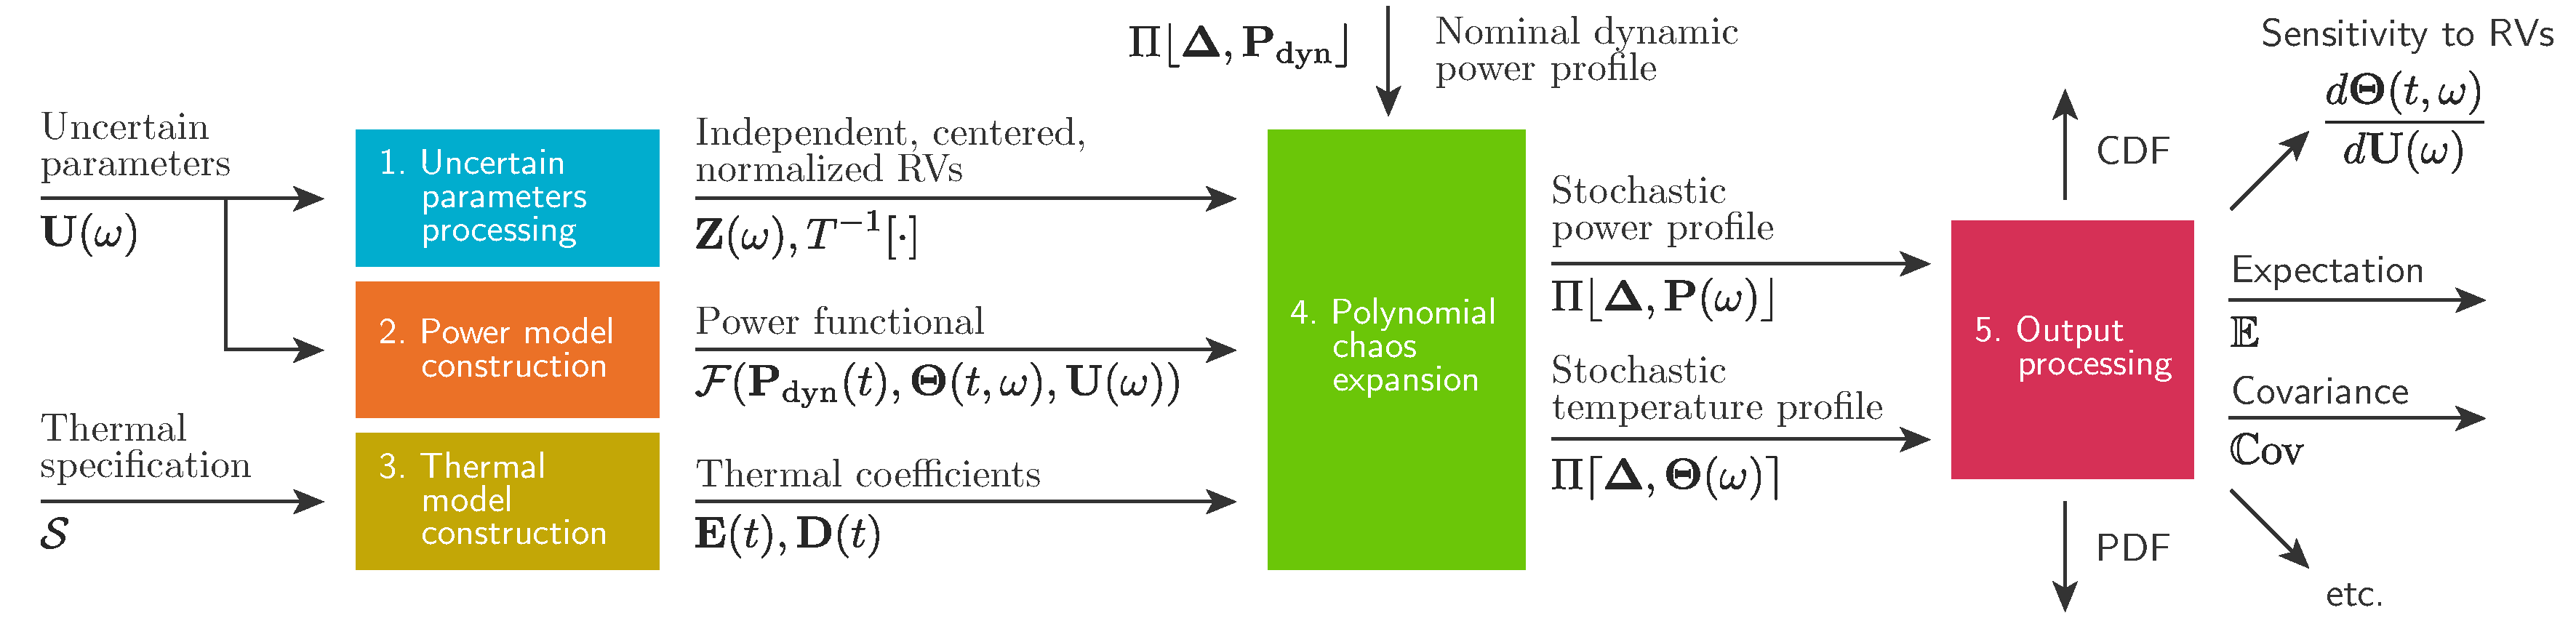
\includegraphics[width=0.9\textwidth]{include/assets/algorithm.pdf}
  \vspace{-0.7em}
  \caption{The structure of the proposed framework.}
  \flabel{algorithm}
  \vspace{-1.6em}
\end{figure*}

The probability space that we shall reside in is defined as a triple $(\outcomes, \sAlgebra, \pMeasure)$ where $\outcomes$ is a set of outcomes, $\sAlgebra \subseteq 2^\outcomes$ is a $\sigma$-algebra on $\outcomes$, and $\pMeasure: \sAlgebra \to [0, 1]$ is a probability measure \cite{maitre2010}.
Loosely speaking, an $n$-dimensional random variable is then a mapping $\v{X}: \o \in \outcomes \mapsto \v{X}(\o) \in \real^n$.
In what follows, the probability space $(\outcomes, \sAlgebra, \pMeasure)$ is always implied.

Consider a heterogeneous multiprocessor system that consists of $\nprocs$ processing elements and is equipped with a thermal package.
The processing elements are the active components of the system, \ie, those that dissipate power, identified at the intended level of granularity (processors, ALUs, caches, registers, \etc).
Let $\system$ be a thermal specification of the system defined as a collection of temperature-related information: (a) the floorplans of the active layers of the chip; (b) the geometry of the thermal package; and (c) the thermal parameters of the materials that the chip and package are made of.

A (transient) power profile $\profileP$ is defined as a tuple composed of a data matrix $\mP = (\vP_i) \in \real^{\nprocs \times \nsteps}$, $\vP_i \in \real^\nprocs$, that captures the power dissipation of the $\nprocs$ processing elements at $\nsteps$ moments of time and a (column) vector $\partition{\mP} = (\t_i) \in \real^{\nsteps}$ with positive and strictly increasing components that specifies these moments of time.
The definition of a (transient) temperature profile $\profileT$ is the same as the one for power except that the data matrix $\mTO$ contains temperature.

The system is assumed to depend on a set of uncertain parameters, denoted by a random vector $\vU(\o)$, $\o \in \outcomes$, which manifest themselves in deviations of the actual power dissipation from nominal values and, consequently, in deviations of temperature from the one corresponding to the nominal power consumption.
In what follows, we shall make a distinction between deterministic and stochastic profiles.
In the latter case, the power and temperature profiles are denoted by $\profileP{\o}$ and $\profileT{\o}$, respectively.

The goal of this work is to develop a probabilistic framework for power-temperature analysis (PTA) of multiprocessor systems where the actual power dissipation and temperature are stochastic due to their dependency on the set of uncertain parameters $\vU(\o)$.
The user is required to: (a) provide a thermal specification of the platform $\system$; (b) have prior knowledge (or belief) on the probability distribution of the uncertain parameters (\sref{uncertain-parameters}); and (c) specify a power model, in which $\vU(\o)$ is an input (\sref{power-model}).
The framework should provide the user with the tools to analyze the system under an arbitrary given workload and obtain the corresponding stochastic power $\profileP{\o}$ and temperature $\profileT{\o}$ profiles with a desired level of accuracy and at low costs.
